
\chapter[Referencial Teórico]{Referencial Teórico}
Este capítulo apresenta os conceitos teóricos que abordam este trabalho, detalhando a estrutura cerebral responsável pela geração dos sinais de interesse na subseção 2.1, o sistema de captura dos sinais (a EEG) na subseção 2.2, o sistema que se refere às BCIs que realizam a tradução dos sinais em comandos para dispositivos na subseção 2.3, os detalhes técnicos a respeito dos sinais oferecidos pela base de dados \textit{BCI Competition} na subseção 2.4, a estrutura geral de um classificador LDA na subseção 2.5, os conceitos de um SoC na subseção 2.6 e por fim o estado da arte das implementações de algoritmos de classificação na subseção 2.7. 

\section{O Cérebro}
O Sistema Nervoso Central (SNC) é o responsável direto pelo comando do nosso comportamento geral\cite{David_Clarck}. Ele pode ser dividido em três principais áreas: tronco encefálico ou medula espinhal, o cérebro e o cerebelo (Figura \ref{BrainParts}) \cite{alvarezneurobiomecanismos}.

\begin{figure}[h]
	\centering
	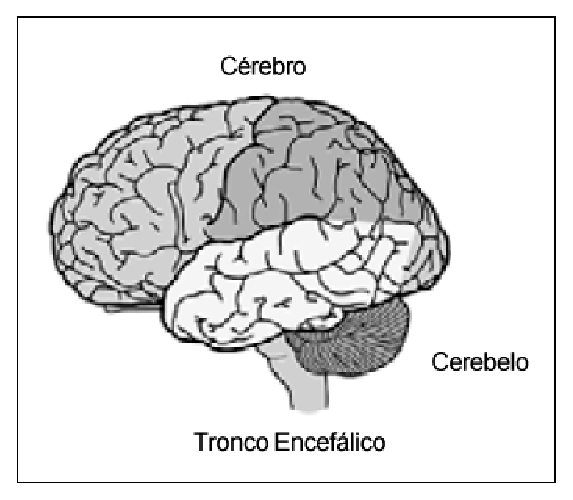
\includegraphics[keepaspectratio=true,scale=1.0]{figuras/estrutura_cerebral.eps}
	\caption{Três principais áreas do cérebro \cite{alvarezneurobiomecanismos}}
	\label{BrainParts}
\end{figure}

O tronco encefálico, parte caldal do SNC recebe e processa todos os sinais dos sensores corporais, além de realizar o controle dos membros e do tronco humano \cite{KANDEL}.

O cérebro é o processador do SNC, nele são recebidos e processados os sinais da medula espinhal, além de fornecer todos os sinais de controle para a própria medula, que por sua vez distribui os sinais para os membros e tronco \cite{KANDEL}.

O cerebelo é localizado logo atrás do tronco encefálico que se conectam através de fibras chamadas de pedúnculos \cite{KANDEL}, é a segunda maior estrutura do SNC contendo mais da metade dos neurônios cerebrais, \cite{SIULYDissertacao} é responsável pelo mapeamento em volta do indivíduo, ou seja, sua percepção \cite{alvarezneurobiomecanismos}, além do controle da região motora e a memória de movimentos \cite{SIULYDissertacao,alvarezneurobiomecanismos}

Os sinais de controle e de sensoriamento são sinais elétricos armazenados nos neurônios \cite{KANDEL}. Suas características eletroquímicas permitem que os neurônios armazenem e transmitam sinais elétricos para qualquer outra célula receptora mesmo que a longa distâncias \cite{SIULYDissertacao}. Sua estrutura pode ser dividida em três principais partes: 1) Corpo da celula, 2) axônio e 3) dendrito, conforme apresentado na Figura(\ref{neuronParts}).
\begin{figure}[h]
	\centering
	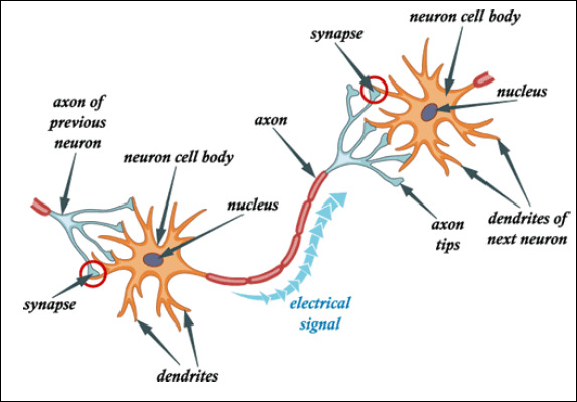
\includegraphics[keepaspectratio=true,scale=1.0]{figuras/Estrutura_neuronio.PNG}
	\caption{Estrutura de um neurônio \cite{SIULYDissertacao}}
	\label{neuronParts}
\end{figure}

A ativação dos neurônios é dada através de um gradiente de concentração eletroquímico, resultando na produção de uma corrente elétrica cerebral que flui através do axônio, o que torna possível a comunicação com outras celulas \cite{SIULYDissertacao}. A corrente elétrica cerebral consiste comumente de íons de Na+, K+, Ca++ e Cl- \cite{EEGSignals}.

As atividades elétricas cerebrais podem ser divididas em dois conjuntos: os potenciais de ação (AP) e os potenciais de sinapse (SP) \cite{SIULYDissertacao}.

Sempre que um potencial de sinapse atinge o limite de condução, ou seja, se o potencial é carregado (estimulado por algua atividade cerebral) até o ponto em que se é gerada uma corrente elétrica no axônio, um AP é iniciado \cite{SIULYDissertacao}.

Como dito antes, o cerebelo é o responsável pelo controle da percepção e dos movimentos, além da memória de movimento, portanto a percepção, os movimentos e a imagética motora são os estímulos que iniciam uma AP na região do cerebelo \cite{alvarezneurobiomecanismos}.

\section{Eletroencefalografia}
A Eletroencefalografia (EEG) é um somatório de potenciais elétricos
 (na faixa de micro volt) representados graficamente em tempo real.
 [MONITORAMENTO DO CÉREBRO COM ELETROENCEFALOGRAFIA E O ÍNDICE BISPECTRAL
 DERIVADO DO ELETROENCEFALOGRAMA DURANTE A CIRURGIA CARDÍACA], esses potenciais
 refletem a atividade elétrica do cérebro humano. É muito usado por profissionais
 de saúde e cientistas para avaliar e estudar funções cerebrais e diagnosticar
 disturbios neurológicos.[LIVRO BCI] 

A técnica popular que registra sinais do cérebro usando eletrodos estratégicamente
 colocados sobre o couro cabeludo do paciente portanto, não invasiva, é muito
 importante nos diagnósticos de doenças neurológicas. Em um exame de EEG ,
 dependendo da sua aplicação, podem ser usados de 1 a 256 eletrodos que iram
 captar os sinais de forma paralela, cada par de eletrodos é chamado de um canal,
 portanto com 256 eletrodos tem-se uma leitura de 128 canais, também conhecido como
 EEG multicanais, cada canal recebe um amplificador de instrumentação e a um equipamento
 de gravação do EEG.

Devido às diferentes camadas e tecidos interpostos entre a fonte do sinal
 (atividade neural no córtex) e os sensores colocados no couro cabeludo,
 tudo isso atuando como um filtro passa-baixa, faz com o que a resolução
 espacial do EEG seja ruim.[RAO R.P.N.-BRAIN-COMPUTER INTERFACING AN
 INTRODUCTION-CAMBRIDGE UNIVERSITY PRESS (2013)], em contra partida a
 resolução temporal é boa, na casa de milessegundos.

Com a baixa amplitude desse tipo de sinal, ele pode sofrer facilmente
 atenuações, contaminações em seu espectro, como por exemplo interferência
 da rede elétrica de 60 Hz e seus harmônicos associados, e principalmente
 atividades musculares exercidas no ato da extração dos sinais. Portanto
 no momento do exame os pacientes são orientados a não realizar nenhum
 tipo de movimento. A instrumentação eletrônica faz um grande trabalho
 ao usar filtros e algoritmos que ptoporcionam a visualização e leitura
 desses sinais por um especialista da área.

\section{\textit{Brain Computer Interface}}

\section{\textit{BCI Competition}}
A \textit{BCI Competition} é uma competição que promove o desenvolvimento e melhoria da tecnologia voltada para as BCIs, onde são submetidas diferentes técnicas de análise de dados cerebrais \cite{BCICompetition}. Já foram realizadas quatro edições da competição, nos anos de 2001, 2002, 2004 e 2008 \cite{BCICompetition}. Em cada uma destas competições são fornecidos publicamente sinais cerebrais, adquiridos em laboratórios especializados \cite{BCICompetition}. Estes sinais são divididos em dois conjuntos de dados, os dados de treinamento e os dados de teste, que são utilizados para treinamento e teste dos algoritmos dos participantes \cite{BCICompetition}.

\subsection{\textit{BCI Competition III}}
O objetivo do \textit{BCI Competition III} é validar as metodologias de classificação e processamento de sinais cerebrais aplicados em BCIs desenvolvidas pelos participantes da competição \cite{siteBCI}. Esta edição foi realizada entre Maio e Junho de 2004, onde foram disponilizados 8 \textit{datasets} (I, II, II, IIIa, IIIb, IVa, IVb, IVc e V), desenvolvidos com a participação de 49 laboratórios especializados \cite{BCICompetition}.
Para cada um dos \textit{datasets} foram realizadas diferentes tarefas que estimulam atividades cerebrais durante a aquisição dos sinais, configurando assim um objetivo especifico para cada um dos \textit{datasets} \cite{siteBCI}.

\subsection{\textit{BCI Competition III - Dataset IVa}}
O \textit{dataset IVa} refere-se a um conjunto de dados adquiridos através da EEG, onde os sujeitos (indivíduos nos quais foram capturados os sinais) foram submetidos a estimular o cérebro por imagética motora, através de indicações visuais \cite{BCICompetition}. Os indivíduos foram submetidos a realizarem três tarefas, indicadas visualmente por 3.5s cada tarefa, sendo interrompidas em periodos aleatórios entre 1.75s e 2.25s, onde o sujeito era submetido a um periodo de relaxamento \cite{BCICompetition}. As três tarefas de imagéticas motoras foram: (L) mão esquerda, (R) mão direita e (F) pé direito \cite{BCICompetition}.

Foram adquiridos sinais de 5 sujeitos rotulados em \textit{aa, al, av, aw} e \textit{ay}, onde foram executadas no total 280 tarefas por cada sujeito, algumas previamente rotulada (dados de treinamento) em cada instante de tempo onde a tarefa foi executada, outras não rotuladas (dados de teste) \cite{siteBCI}. Estes sinais foram adquiridos, tratados e disponibilizados por \textit{Fraunhofer FIRST, Intelligent Data Analysis Group (Head: Klaus-Robert Müller), and Charité University Medicine Berlin, Campus Benjamin Franklin, Department of Neurology, Neurophysics Group} \cite{BCICompetition}. A tabela 1 apresenta a quantidade de tarefas previamente classificadas (nomeados \#tr) e a quantidade de tarefas não classificadas (nomeadas \#te) para cada sujeito.

\begin{table}[h!]
	\centering
	\caption{Número de tarefas rotuladas e não rotuladas por sujeito \cite{BCICompetition}.}
	\label{my-label}
	\begin{tabular}{lll}
		\textbf{Sujeitos} & \textbf{\#tr} & \textbf{\#te} \\
		\textit{aa} & 168 & 112 \\
		\textit{al} & 224 & 56 \\
		\textit{av} & 84 & 196 \\
		\textit{aw} & 56 & 224 \\
		\textit{ay} & 28 & 252
	\end{tabular}
\end{table}
 
\section{\textit{Linear Discriminant Analisys}}
Supondo a existência de um conjunto de dados $\vec x$,com características multivariadas, e que cada dado
seja conhecido devido ser proveniente de uma das  classes $y$, tal que são predefinidas com características
semelhantes aos dados. As classes podem ser exemplificadas como sendo: espécies de plantas,
precença ou ausência de uma condição médica específica, diferentes tipos de tumores, tipos de veículos automotores
entre outros. Para separar as classes conhecidas uma das outras, é atribuido um rótulo a cada classe, então os dados são
representados como dados rotulados \cite{izenmanLDA}.


Devido a indispensabilidade de diminuir as dimensões dos dados de um determinado conjunto, o objetivo do LDA
é reduzir a dimensão do espaço de conjunto de dados, resolvendo o inconvêniente da sobreposição \cite{SinghLDA}.

No reconhecimento de padrões supervisionados, o classificador é desenvolvido explorando as informações 
já conhecidas e contidas num vetor de treinamento disponibilizado préviamente\cite{izenmanLDA}. O LDA tem a 
proposta de encontrar uma transformação ótima para maximizar a proporção de acordo com a equação \ref{eq: Proporção}.
\begin{equation}
	\label{eq: Proporção}
	J(W) = \frac { W^T S_B W}{W^T S_W W}
\end{equation}

Onde $S_B$ é a matriz de dispersão entre as classes e$ S_W$ a matriz de dispersão dentro das classes. 

Quando o número de classes a serem separadas são apenas duas, assume-se que as funções de probabilidade
são normalmente distribuidas

\section{\textit{System-on-Chip}}

\textit{System-on-Chip} (SoC), implica que todo sistema que contém funcionalidades implementadas em hardware e software se encontra em um único chip de silício,combinando processamento, lógica de alta velocidade, interface, memória entre outros componentes ao invés de uma implementação maior em vários chips físicos diferentes agrupados em uma placa 
de cicuito impresso \cite{zynqBook}.

São vários os argumentos a favor da escolha de um SoC a uma placa de circuito impresso, pode-se citar que a solução é de menor custo, viabiliza transferência de dados mais rápidas e seguras entre vários elementos do sistema, possui maior velocidade geral do sistema, menor consumo de energia entre vários outros elementos que fortalecem a escolha de um SoC em sistemas discretos com componentes equivalentes \cite{zynqBook}.

\subsection{Aquitetura Simplificada de um SoC}

O conjunto da aquitetura pode se dividir em dois sistemas, sistema de
hardware  e sistema de software. 


No \textbf{Sistema de Hardware}
encontram-se todos os periféricos,
memórias e processadores, para conecta-los
existe um barramento de comunicação
responsável por isso.
Já no \textbf{Sistema de Software}, o software é do tipo stack, e funciona sobre o
processador, que também sustenta os aplicativos que geralmente têm um
Sistema Operacional (SO) para gerência, uma camada em um nível mais baixo
faz a interface com o sistema de hardware \cite{zynqBook}.

 Diagrama
\subsection{\textit{Zybo-Board}}
A Zybo é uma plataforma de desenvolvimento(figura\ref{Zybo Board}), que é equipada com o Z-7010
este que é  o menor integrante da familía Xilinx Zynq-7000.
Baseado na arquitetura Xilinx$^{\textregistered}$ \textit{All-Programmable System-on-Chip} (AP SoC)
o Z-7010 possui em seu encapsulamento um processador ARM Cortex-A9 de 
dois núcleos e um Xilinx 7-Series(FPGA), Esse chip combinado com memórias, entradas 
e saídas de áudio e vídeo, USB, Ethernet, slot SD entre outros periféricos e suportes
proporciona um \textit{kit} para desenvolvedores que procuram uma plataforma de baixo custo
sem perder a capacidade de processamento do Zynq AP SoC. (store Digilent)  

\begin{figure}[h]
	\centering
	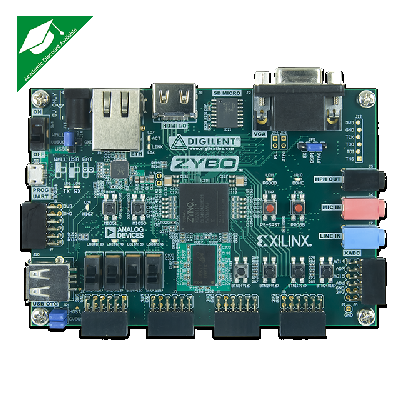
\includegraphics[keepaspectratio=true,scale=1.0]{figuras/zyboboard.eps}
	\caption{Placa de Desenvolvimento Zybo-Board}
	\label{Zybo Board}
\end{figure}



\section{Estado da Arte}



